\chapter{Backend SDK}

Appsemble werkt met extensions, individueel ontwikkelde componenten, om een app te maken. Extensions worden ontwikkeld door d-centralize zelf, en hopelijk in de toekomst door externe ontwikkelaars buiten het bedrijf. \\

Dit moet echter allemaal weergegeven worden. De ontwikkelaar moet namelijk complete vrijheid hebben om een extension te ontwikkelen met de tools die hij/zij wilt. Dit betekent dat er een geunificeerde oplossing moet zijn voor het laden van extensions. \\ 

In appsemble wordt dit geregeld met iframes. Dit is een html element waarin een nieuwe webpagina geladen word. Ontwikkelaars moeten een extension dan ook eerst registreren bij de appsemble-api. Vanaf dit punt verschijnt het in de lijst met componenten. \\

Dit zorgt er echter voor dat een developer arbitrair scripts kan injecteren. Het is dus een security risico om developers te laten doen wat zij willen. Hier komt de sdk langs. \\

De sdk verzorgt een middenlaag tussen de extension en de verschillende services die zij willen gebruiken.Dit zorgt ervoor dat de extensions zelf goed beschermd zijn tegen boosdoeners, znder dat er verminderde functionaliteit is.

\section{Requirements}

Om te zorgen dat er ontwikkeld kan worden voor appsemble moet de backend van de sdk netjes ontwikkeld worden. De backend zelf heeft dus ook de volgende requiremenst.

\begin{itemize}
	\item Kan rpc calls afhandelen
	\item Werkt met promises
	\item Kan specifieke functies aanroepen
	\item Is makkelijk uit te breiden
\end{itemize}

Om ervoor te zorgen dat er verschillende functies aangeroepen kunnen worden is er gebruikt gemaakt van een call-register. Dit is een dictionairy die een naam verbind aan een functie\footnote{In javascript zijn functies first-class citizen's en kunnen dus doorgegeven worden aan andere functies}. \\

Dit zorgt ervoor dat, indien de goede naam is gebruikt, de correcte functie zal worden uitgevoerd. Bij een functie call word dan ook een payload meegegeven. Dit is de data die een functie nodig uit te voeren. In feite is zijn het de function parameters, maar dan verpakt in een javascript object. \\

Functies in de sdk worden samengevoegd in klassen, met betrekking tot hun doel. Dit zorgt ervoor dat dezelfde api's altijd in dezelfde klassen zitten. \\

Uiteindelijk worden deze klassen samengevoegd in de sdk, waarbij de sdk aan iedere klasse vraagt welke functies zij aanbieden. Dit word gecombineerd in een groot register, die vervolgens gebruikt wordt voor het aanroepen van zijnde functies. \\

De api's van de sdk kunnen alles wat mogelijk is binnen angular2, zoals het aanroepen van externe api's en het veranderen van de staat van appsemble zelf\footnote{Mits hier een functie voor is}.

\begin{figure}[h]
	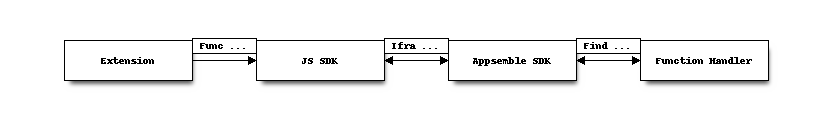
\includegraphics[width=1\textwidth]{diagrams/sdk-call.png}	
	\caption{\textit{Het schema van een sdk call}}
\end{figure}
\section{Geschreven sdk componenten}

\subsection{Resources}

De resource api biedt de mogelijkheid voor developers om data te lezen en te schrijven. Het word gebackt door de google cloud database. Ontwikkelaars kunnen door middel van resource configurations zelf een tabel aanmaken in deze database. Vervolgens kan met een simpele sdk call hier data naar geschreven worden.